\documentclass[border=5pt]{standalone}
\usepackage{fontspec}
\usepackage{unicode-math}
\setmainfont{Noto Serif}
\newfontfamily\FigureItalic{Noto Serif}
\setmathfont{STIXTwoMath-Regular.otf}
\usepackage{tikz}
\usetikzlibrary{arrows.meta,calc,patterns,decorations.pathmorphing,decorations.markings,decorations.pathreplacing,positioning,backgrounds}
\definecolor{Ink}{HTML}{000000}
\definecolor{Curve}{HTML}{000000}
\definecolor{Bzero}{HTML}{000000}
\definecolor{Bone}{HTML}{000000}
\definecolor{Btwo}{HTML}{000000}
\definecolor{Bthree}{HTML}{000000}
\definecolor{Bfour}{HTML}{000000}
\tikzset{
 ax/.style={draw=Ink,line width=.72pt,-{Latex[length=2.4mm,width=1.5mm]}},
 lev/.style={draw=Ink,line width=1.4pt,line cap=butt},
 thinlev/.style={draw=Ink,line width=.65pt,line cap=butt},
 helper/.style={draw=Ink,line width=.65pt},
 bare/.style={draw=Ink,line width=.95pt,dash pattern=on 4pt off 2.8pt},
 curve/.style={draw=Ink,line width=1.85pt,line cap=round,line join=round},
 ray/.style={draw=Ink,line width=1.0pt,-{Latex[length=2.3mm,width=1.4mm]}},
 measure/.style={draw=Ink,line width=.75pt,{Latex[length=1.9mm,width=1.2mm]}-{Latex[length=1.9mm,width=1.2mm]}},
 link/.style={draw=Ink,line width=1.0pt},
 wave/.style={draw=Ink,line width=.85pt,decorate,decoration={snake,amplitude=.33mm,segment length=2.5mm,pre length=.8mm,post length=.8mm}},
 photon/.style={draw=Ink,line width=1.0pt,-{Latex[length=2.0mm,width=1.3mm]},decorate,decoration={snake,amplitude=.4mm,segment length=2.7mm,pre length=0mm,post length=1.9mm}},
 lab/.style={text=Ink,font=\fontsize{13.5}{16}\selectfont,inner sep=2pt},
 small/.style={text=Ink,font=\fontsize{11.5}{14}\selectfont,inner sep=2pt},
 tag/.style={text=Ink,font=\fontsize{14}{17}\selectfont\FigureItalic\itshape,inner sep=2pt}}
\pagestyle{empty}

\begin{document}
% Figure 12.2; source-grounded revision.
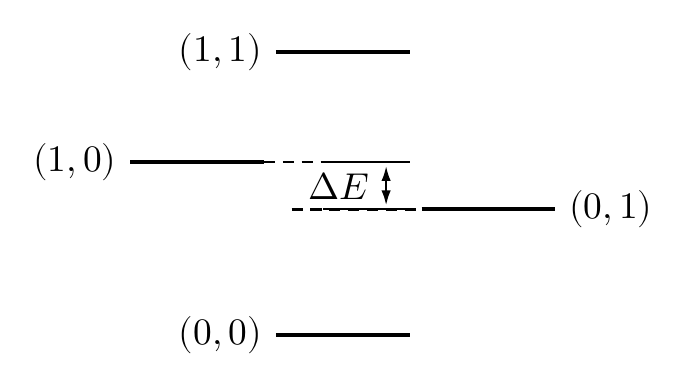
\begin{tikzpicture}[x=1cm,y=1cm]
\coordinate (C11) at (3.00000,4.05000);
\coordinate (C11L) at (2.15000,4.05000);
\coordinate (C11R) at (3.85000,4.05000);
\draw[lev] (C11L) -- (C11R);
\node[lab,anchor=east] at (2.05000,4.05000) {$(1,1)$};
\coordinate (C10) at (1.15000,2.65000);
\coordinate (C10L) at (0.30000,2.65000);
\coordinate (C10R) at (2.00000,2.65000);
\draw[lev] (C10L) -- (C10R);
\node[lab,anchor=east] at (0.20000,2.65000) {$(1,0)$};
\coordinate (C01) at (4.85000,2.05000);
\coordinate (C01L) at (4.00000,2.05000);
\coordinate (C01R) at (5.70000,2.05000);
\draw[lev] (C01L) -- (C01R);
\node[lab,anchor=west] at (5.80000,2.05000) {$(0,1)$};
\coordinate (C00) at (3.00000,0.45000);
\coordinate (C00L) at (2.15000,0.45000);
\coordinate (C00R) at (3.85000,0.45000);
\draw[lev] (C00L) -- (C00R);
\node[lab,anchor=east] at (2.05000,0.45000) {$(0,0)$};
\draw[bare] (C10R) -- (3.55000,2.65000);
\draw[bare] (2.35000,2.05000) -- (C01L);
\draw[measure,line width=.77pt] (3.55,2.10)--(3.55,2.60);
\draw[helper] (2.75,2.65)--(3.85,2.65) (2.75,2.05)--(3.85,2.05);
\node[lab,anchor=east,fill=white,inner sep=1.0pt] at (3.35,2.35) {$\Delta E$};\end{tikzpicture}

\end{document}
